
\documentclass[journal]{IEEEtran}
\usepackage[section]{placeins}
\usepackage{blindtext}
\usepackage{graphicx}
\usepackage{caption}
\usepackage{amsmath}

\ifCLASSINFOpdf
\else
\fi
\hyphenation{Gender Identification}


\begin{document}
	%
	% paper title
	\title{Gender Identification}
	
	\author{Aatman Dholakia,~\IEEEmembership{1401013},
		Rajat Barot,~\IEEEmembership{1401045},
		Charvik Patel,~\IEEEmembership{1401079}, 
		Anuj Shah,~\IEEEmembership{1401084}}
	
	
	
	
	% make the title area
	\maketitle
	
	
	\begin{abstract}
		%\boldmath
		Machine Learning is being used widely in diverse areas such as fraudulent systems, recommender systems, disease prediction, etc. One such application is gender identification which is exploited in this paper. For gender identification it is necessary to extract features of face. The proposed algorithm for the same would be YCbCr color space to detect the skin regions in the color image. For facial feature extraction we use Gabor filters at five scales and eight orientations. To solve classification problem we use Adaboost, SVM based classifier.
	\end{abstract}
	\begin{IEEEkeywords}
		Face Detection, Gender Identification, Gabor Filter, Ada-Boost, SVM, Machine learning, classification algorithm
	\end{IEEEkeywords}
	
	
	\IEEEpeerreviewmaketitle
	
	
	
	\section{\textbf{Introduction}}
	Gender Identification has become area of extensive research due to it's increasingly powerful applications. Moreover augmenting it in real time scenario can be useful in many applications in many fields. A successful gender classification could have great impact in improving human computer interactions. Practically it is imperative to improve the algorithms from time to time in order to achieve higher accuracy levels and build more accurate and robust systems.
	
	
	
	
	
	
	
	\ifCLASSOPTIONcaptionsoff
	\newpage
	\fi
	
	
	
	\section{\textbf{METHODOLOGY}}
	Our proposed face detection and sex classification system is
	described in Fig. 1.\\
	\begin{minipage}{\linewidth}
		\centering
		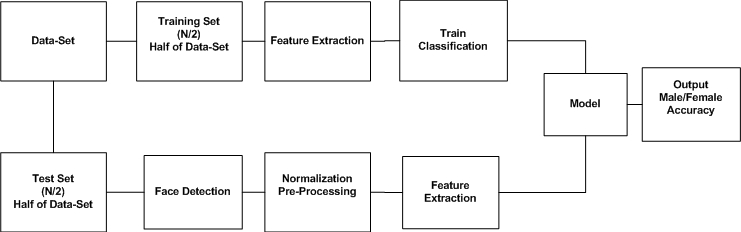
\includegraphics[width = 90mm]{Methodology.JPG}
		\captionof{figure}{Methodology \label{overflow}}
	\end{minipage} 
	
	\section{\textbf{Face Detection}}
	   The proposed algorithm first locates the face region
	using skin-color. The YCbCr color space is used to detect
	the skin region on the given input face image. The given
	input RGB image is converted into the YCbCr color
	space.
	
	
	  Color is a powerful cue of human faces. The
	distribution of skin clusters is in a small region of the
	chromatic color space. Processing color is faster than
	processing other facial features. Therefore, skin color
	detection is firstly performed on the input color image to
	reduce the computational complexity.
	
	In the color detection process, each pixel is classified as
	either skin or non-skin based on its color components.
	 \begin{equation}
	  GammaRGB=(c1*inputRGBimage)^{c21} + c3
	 \end{equation}
	
	where $c1=1.0$, $c2=1.0$ and $c3=0.0$\vspace{1mm}\\
	 
	 The Y, Cb and Cr components are determined through
	the following formula using the constant C with the value
	128. [1]
	\begin{equation}
	\begin{split}
	Y=(0.299*(gammaRGB[0,i,j]-C)+C\\
	+(0.114*(gammaRGB[2,i,j]-C)))
	\end{split}
	\end{equation}
	
	\begin{equation}
	\begin{split}
	Cb=(0.564*(gammaRGB[2,i,j]-Y)
	\end{split}
	\end{equation}
	
	
	\begin{equation}
	\begin{split}
	Cr=(0.713*(gammaRGB[0,i,j]-Y)
	\end{split}
	\end{equation}
	
	 here, gammaRGB is the array with 0 represents the Red
	layer and the 2 represents the Blue layer. The range of Cb
	is between -50 and 2 while the range of Cr is between 10
	and 100 determine the skin region.The skin image is estimated based on the threshold
	gray level between 20 and 80.
	
	\section{\textbf{Facial feature Detection}}
	\begin{enumerate}
	    \item Edge detection is done using Gabor's algorithm which implements linear approach..
	    \item A set of Gabor filters with different frequencies and orientations may be helpful for extracting useful features from an image.
	    \item In the discrete domain, two-dimensional Gabor filters are given by,\\
	    \begin{equation}
	        G_c[i, j] = Be^{(-(x^2+y^2)/2\sigma^2)}cos(2\pi f(icos\theta + jsin\theta))
	    \end{equation}
	    \begin{equation}
	        G_s[i, j] = Ce^{(-(x^2+y^2)/2\sigma^2)}sin(2\pi f(icos\theta + jsin\theta))
	    \end{equation}
	    where B and C are normalizing factors to be determined and f is the frequency being looked for in the texture. $\theta$ is the direction in which feature is to be looked for.
	\end{enumerate}
	
\newpage
\section{\textbf{Result}}
    \begin{minipage}{\linewidth}
		\centering
		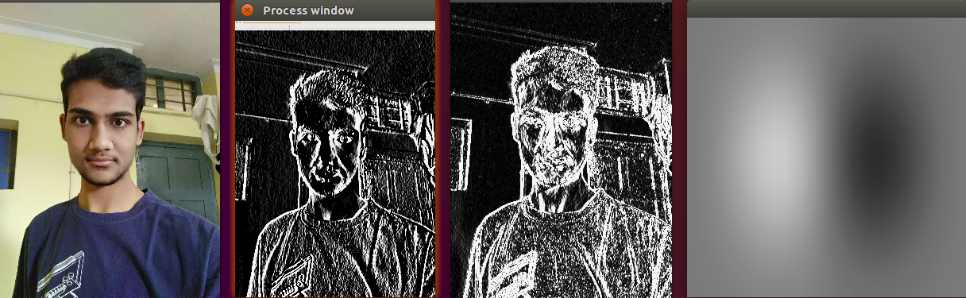
\includegraphics[width = 80mm]{gabor_crop.png}
		\captionof{figure}{Gabor filter for edge detection \label{overflow}}
	\end{minipage} 
	
	\begin{minipage}{\linewidth}
		\centering
		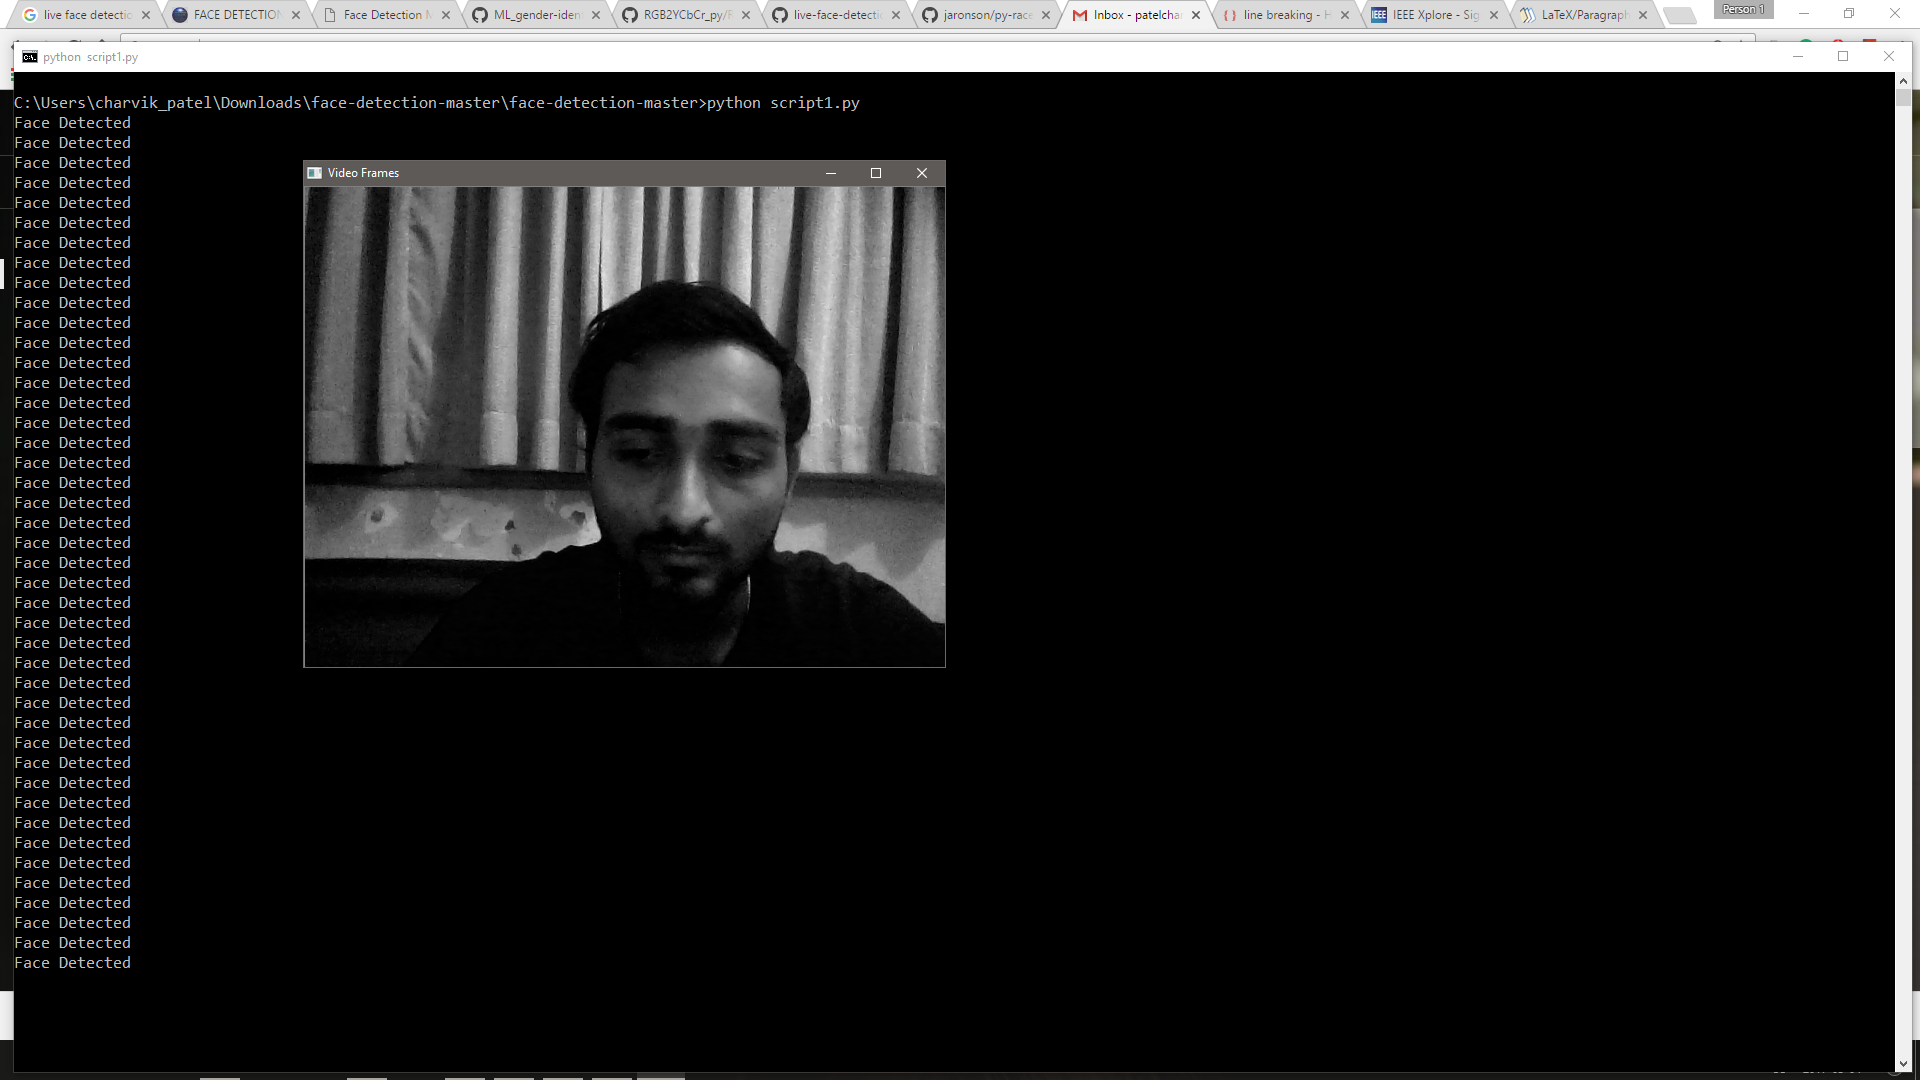
\includegraphics[width = 80mm]{1.png}
		\captionof{figure}{Face Detection Real Time 1 \label{overflow}}
	\end{minipage} 
	
	\begin{minipage}{\linewidth}
		\centering
		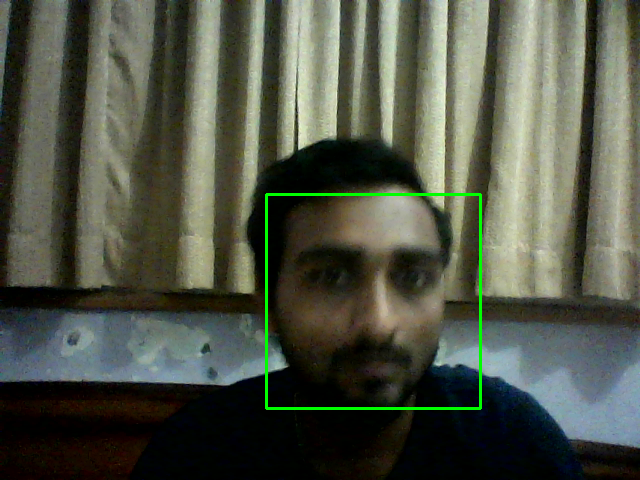
\includegraphics[width = 80mm]{2.png}
		\captionof{figure}{Face Detection Real Time 2 \label{overflow}}
	\end{minipage} 
	
	\begin{minipage}{\linewidth}
		\centering
		
\includegraphics[width = 80mm]{3.png}
		\captionof{figure}{Face Detection Real Time 3 \label{overflow}}
	\end{minipage} 
	
	\section{\textbf{Conclusion}}
	For the Proper Gender Identification we need to Detect the face and need to detect the skin color,facial feature extraction,Geometric Distance between Extracted Feature and need to classify data into two class as follow
	\begin{enumerate}
		\item Male
		\item Female
	\end{enumerate} 
	 
	
	
	
    \section{\textbf{Future Work}}
    \begin{enumerate}
        \item Train classifier to train images for gender classification i.e. person is male or female.
        \item To detect gender of more than one person in real time video at the same time.
        
       
    \end{enumerate}
	
	
	\begin{thebibliography}{1}
	\bibitem{IEEEhowto:kopka}
	“Digital Image Processing”, William K Pratt, Wiley
	Publication, 3rd edition.
	\bibitem{IEEEhowto:kopka}
	"Face Detection with Facial Features and Gender Classification Based On
	Support Vector Machine",S.Ravi,S.Wilson,[publication:2010]
	\bibitem{IEEEhowto:kopka}
	"Gender Detection using Machine Learning Techniques
	and Delaunay Triangulation",Sarthak Gupta[publication:August,2013]
	\bibitem{IEEEhowto:kopka}
	"Face Detection and Sex Identification from Color Images
	using AdaBoost with SVM based Component Classifier",Hafizur Rahman,Tonmoy Das,Manamatha Sarnaker[Publication:August,2013]
	
	\end{thebibliography}
	
	
	
\end{document}


